%DO NOT MESS AROUND WITH THE CODE ON THIS PAGE UNLESS YOU %REALLY KNOW WHAT YOU ARE DOING
\chapter*{Experimental Research}
\addcontentsline{toc}{chapter}{Experimental Research}


\section{ Signal to Noise Ratio } \label{ Signal to Noise Ratio } 
\noindent  The MATLAB program for determining the signal to noise ratio was developed. The following parameter values were considered.

\begin{minipage}[b]{.40\textwidth}
   \centering
   \begin{tabular}{ | l | l |}
     \hline
     \textit{z / r} & uptp 50 m / 600 m \\ \hline
     \textit{bt} & mud, sand and gravel \\ \hline
     \textit{$v_{W}$} & 5, 15 and 25 knots \\ \hline
     \textit{S} & 33 ppt \\ \hline
     \textit{T} & $15^{\circ}$ \\ \hline
     \textit{c} & 1480 m/s \\ \hline
     \textit{SL} & 220 dB \\ \hline
     \textit{f} & 100 kHz \\ \hline
      $ \uptau $& $100 \mu s $\\ \hline
      \textit{DI} & 30 dB \\
     \hline
   \end{tabular}
  \end{minipage}\qquad
\begin{minipage}[b]{.40\textwidth}
   \centering
   \begin{tabular}{ | l | l |}
     \hline
      \textit{B} & 10 kHz \\ \hline
     \textit{$BP_{T}$} & 0 dB $(\pm 90^{\circ})$ \\ \hline
     \textit{$BP_{R}$} & 0 dB $(\pm 90^{\circ})$\\ \hline
     $2\theta_{\textit{h,R}} $ & $0.5^{\circ}$\\ \hline
     $2\theta_{\textit{h,T}} $ & $90^{\circ}$ \\ \hline
     $2\theta_{\textit{v,R}} $ & $180^{\circ}$ \\ \hline
     $2\theta_{\textit{v,T}} $ & $180^{\circ}$ \\ \hline
     \textit{$r_{S}$} & 0 m \\ \hline
      \textit{$z_{S}$} & 5 m \\ \hline
       \textit{TS} & $ -15 dB$ \\
   \hline
   \end{tabular}
   \end{minipage}
   \newpage
   
\noindent Signal to noise ratio (SNR) is a measure of how strong the signal of interest is with respect to the noise environment. The higher the SNR, the better the detection. The Figure 1, Figure 2 and Figure 3 show SNR as a function of depth and range for this particular sonar/environment scenario. In the images, colour is mapped to SNR where red is high and blue is low.

\begin{figure}[h]
\centering
\subfloat[Wind speed = 5 kn]{
  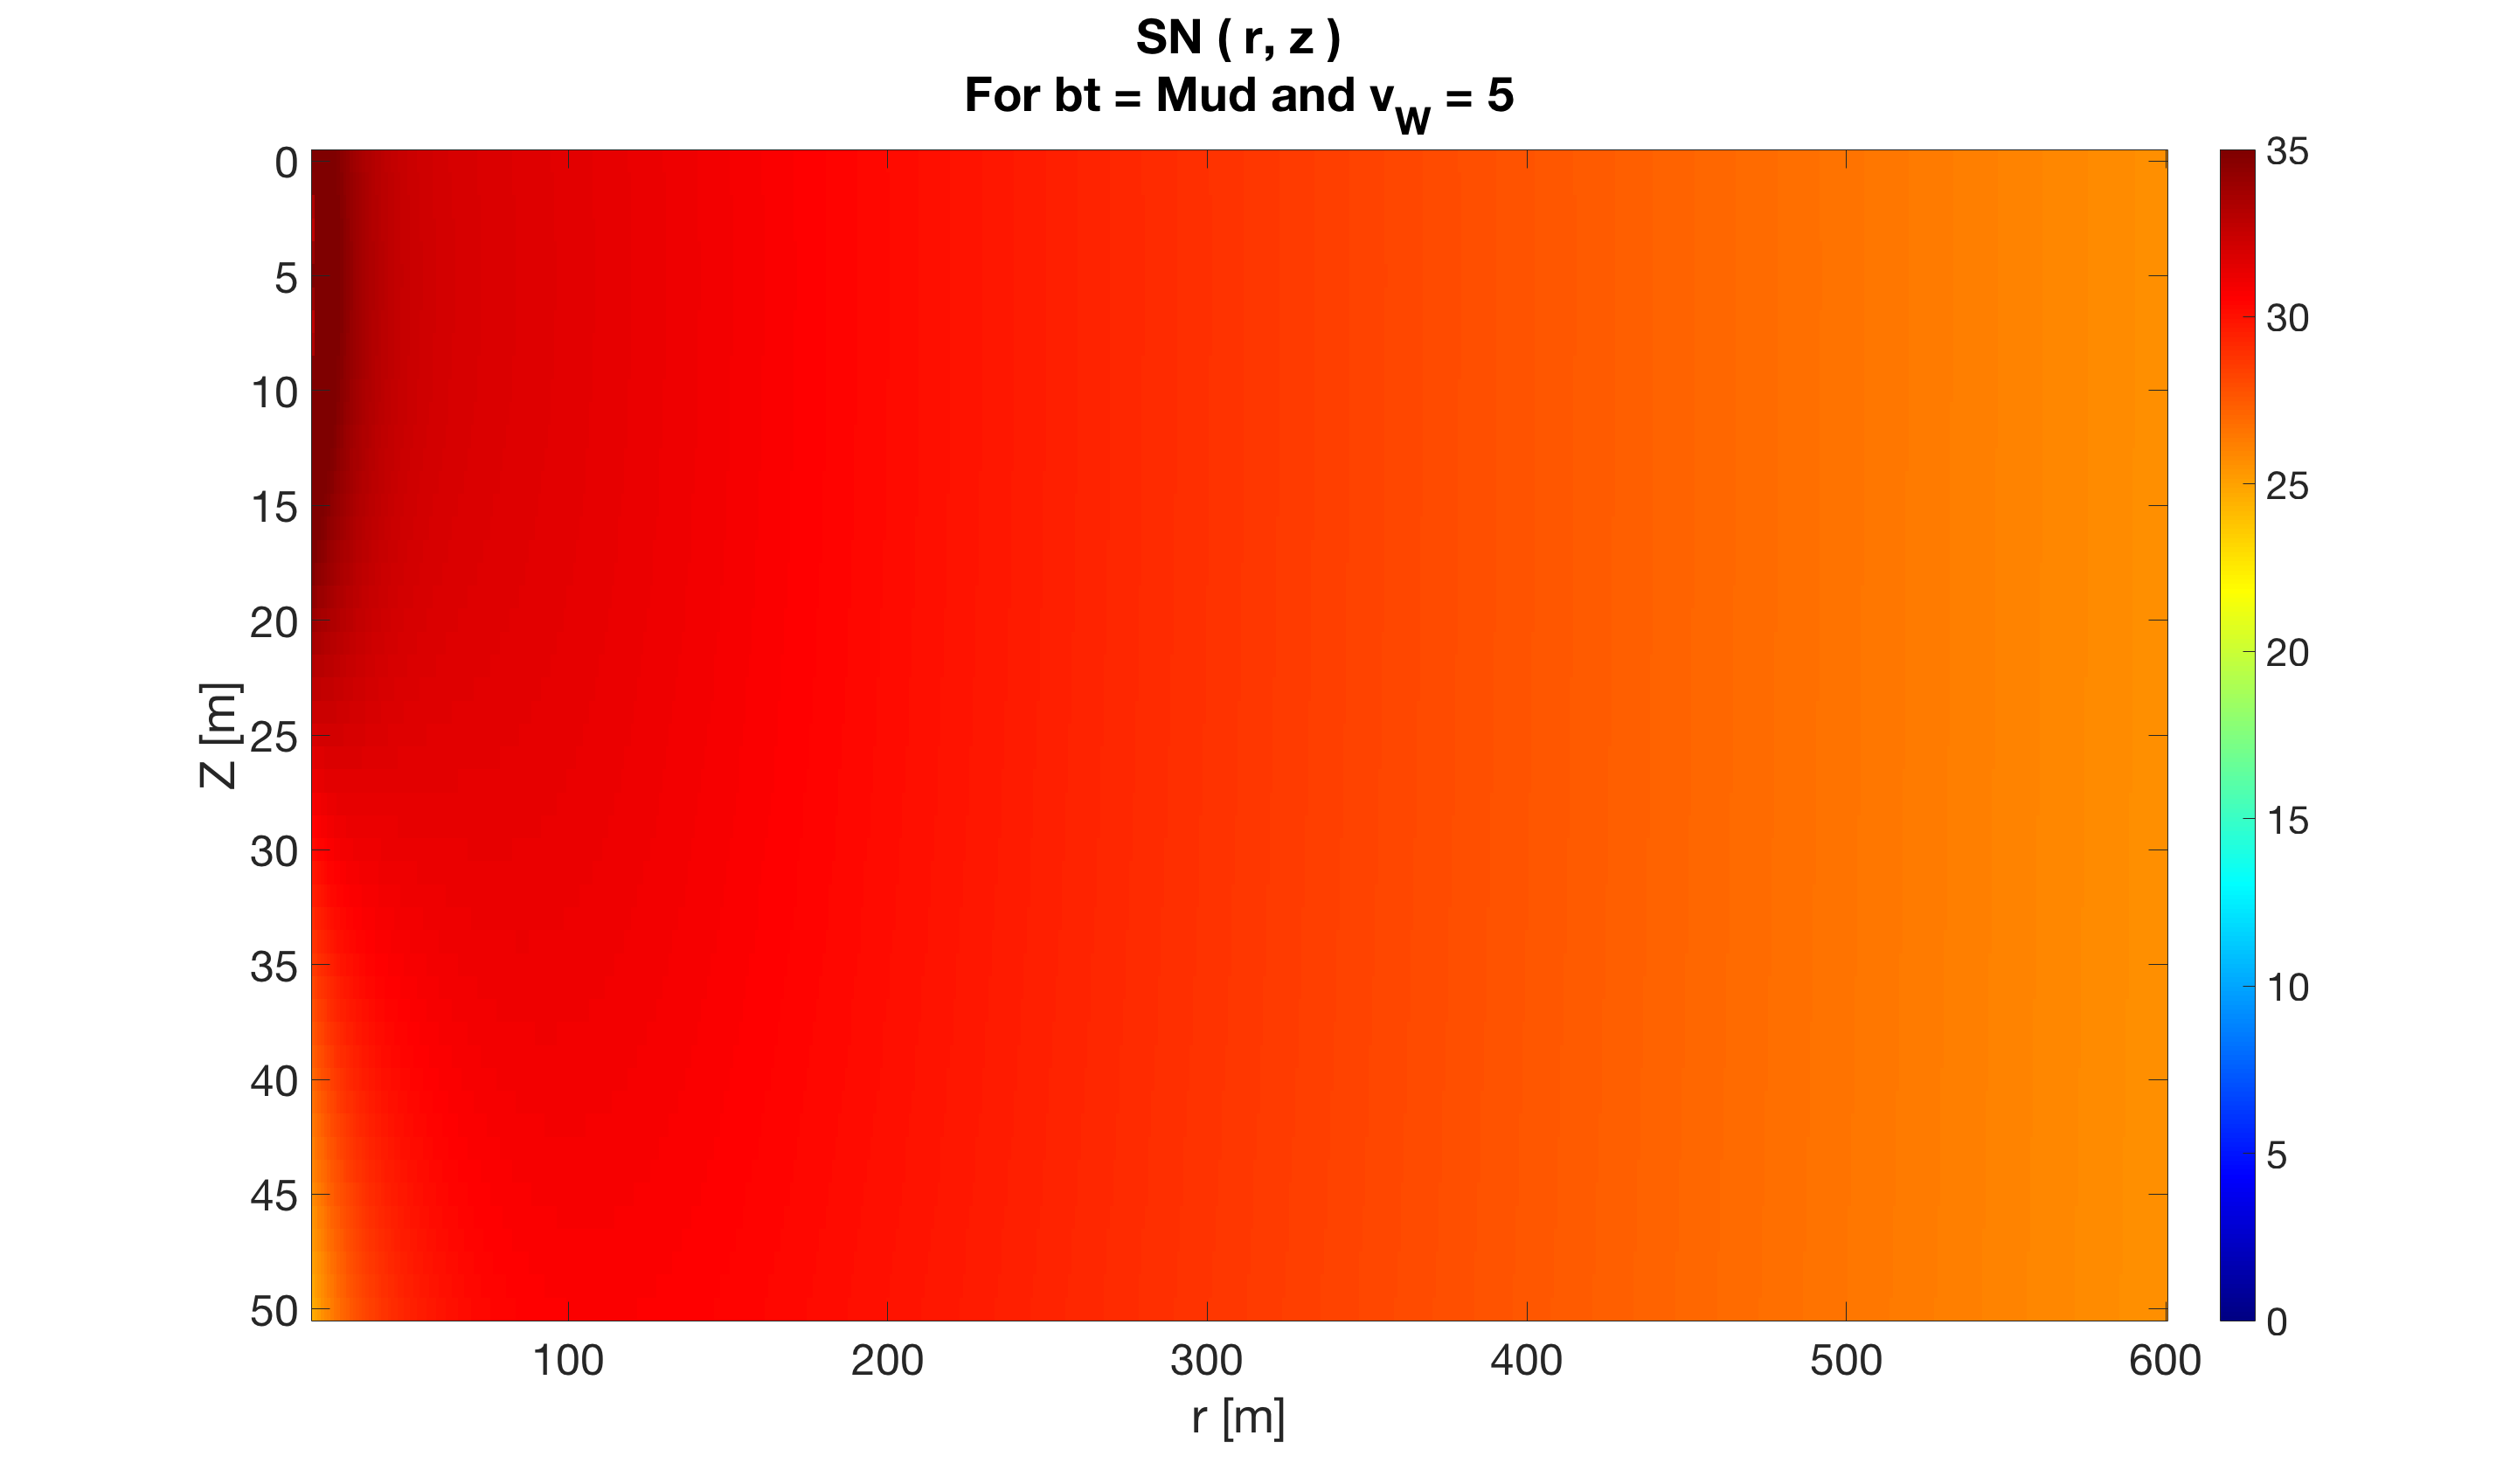
\includegraphics[width=95mm]{fig1.png}
}
\subfloat[Wind speed = 15 kn]{
  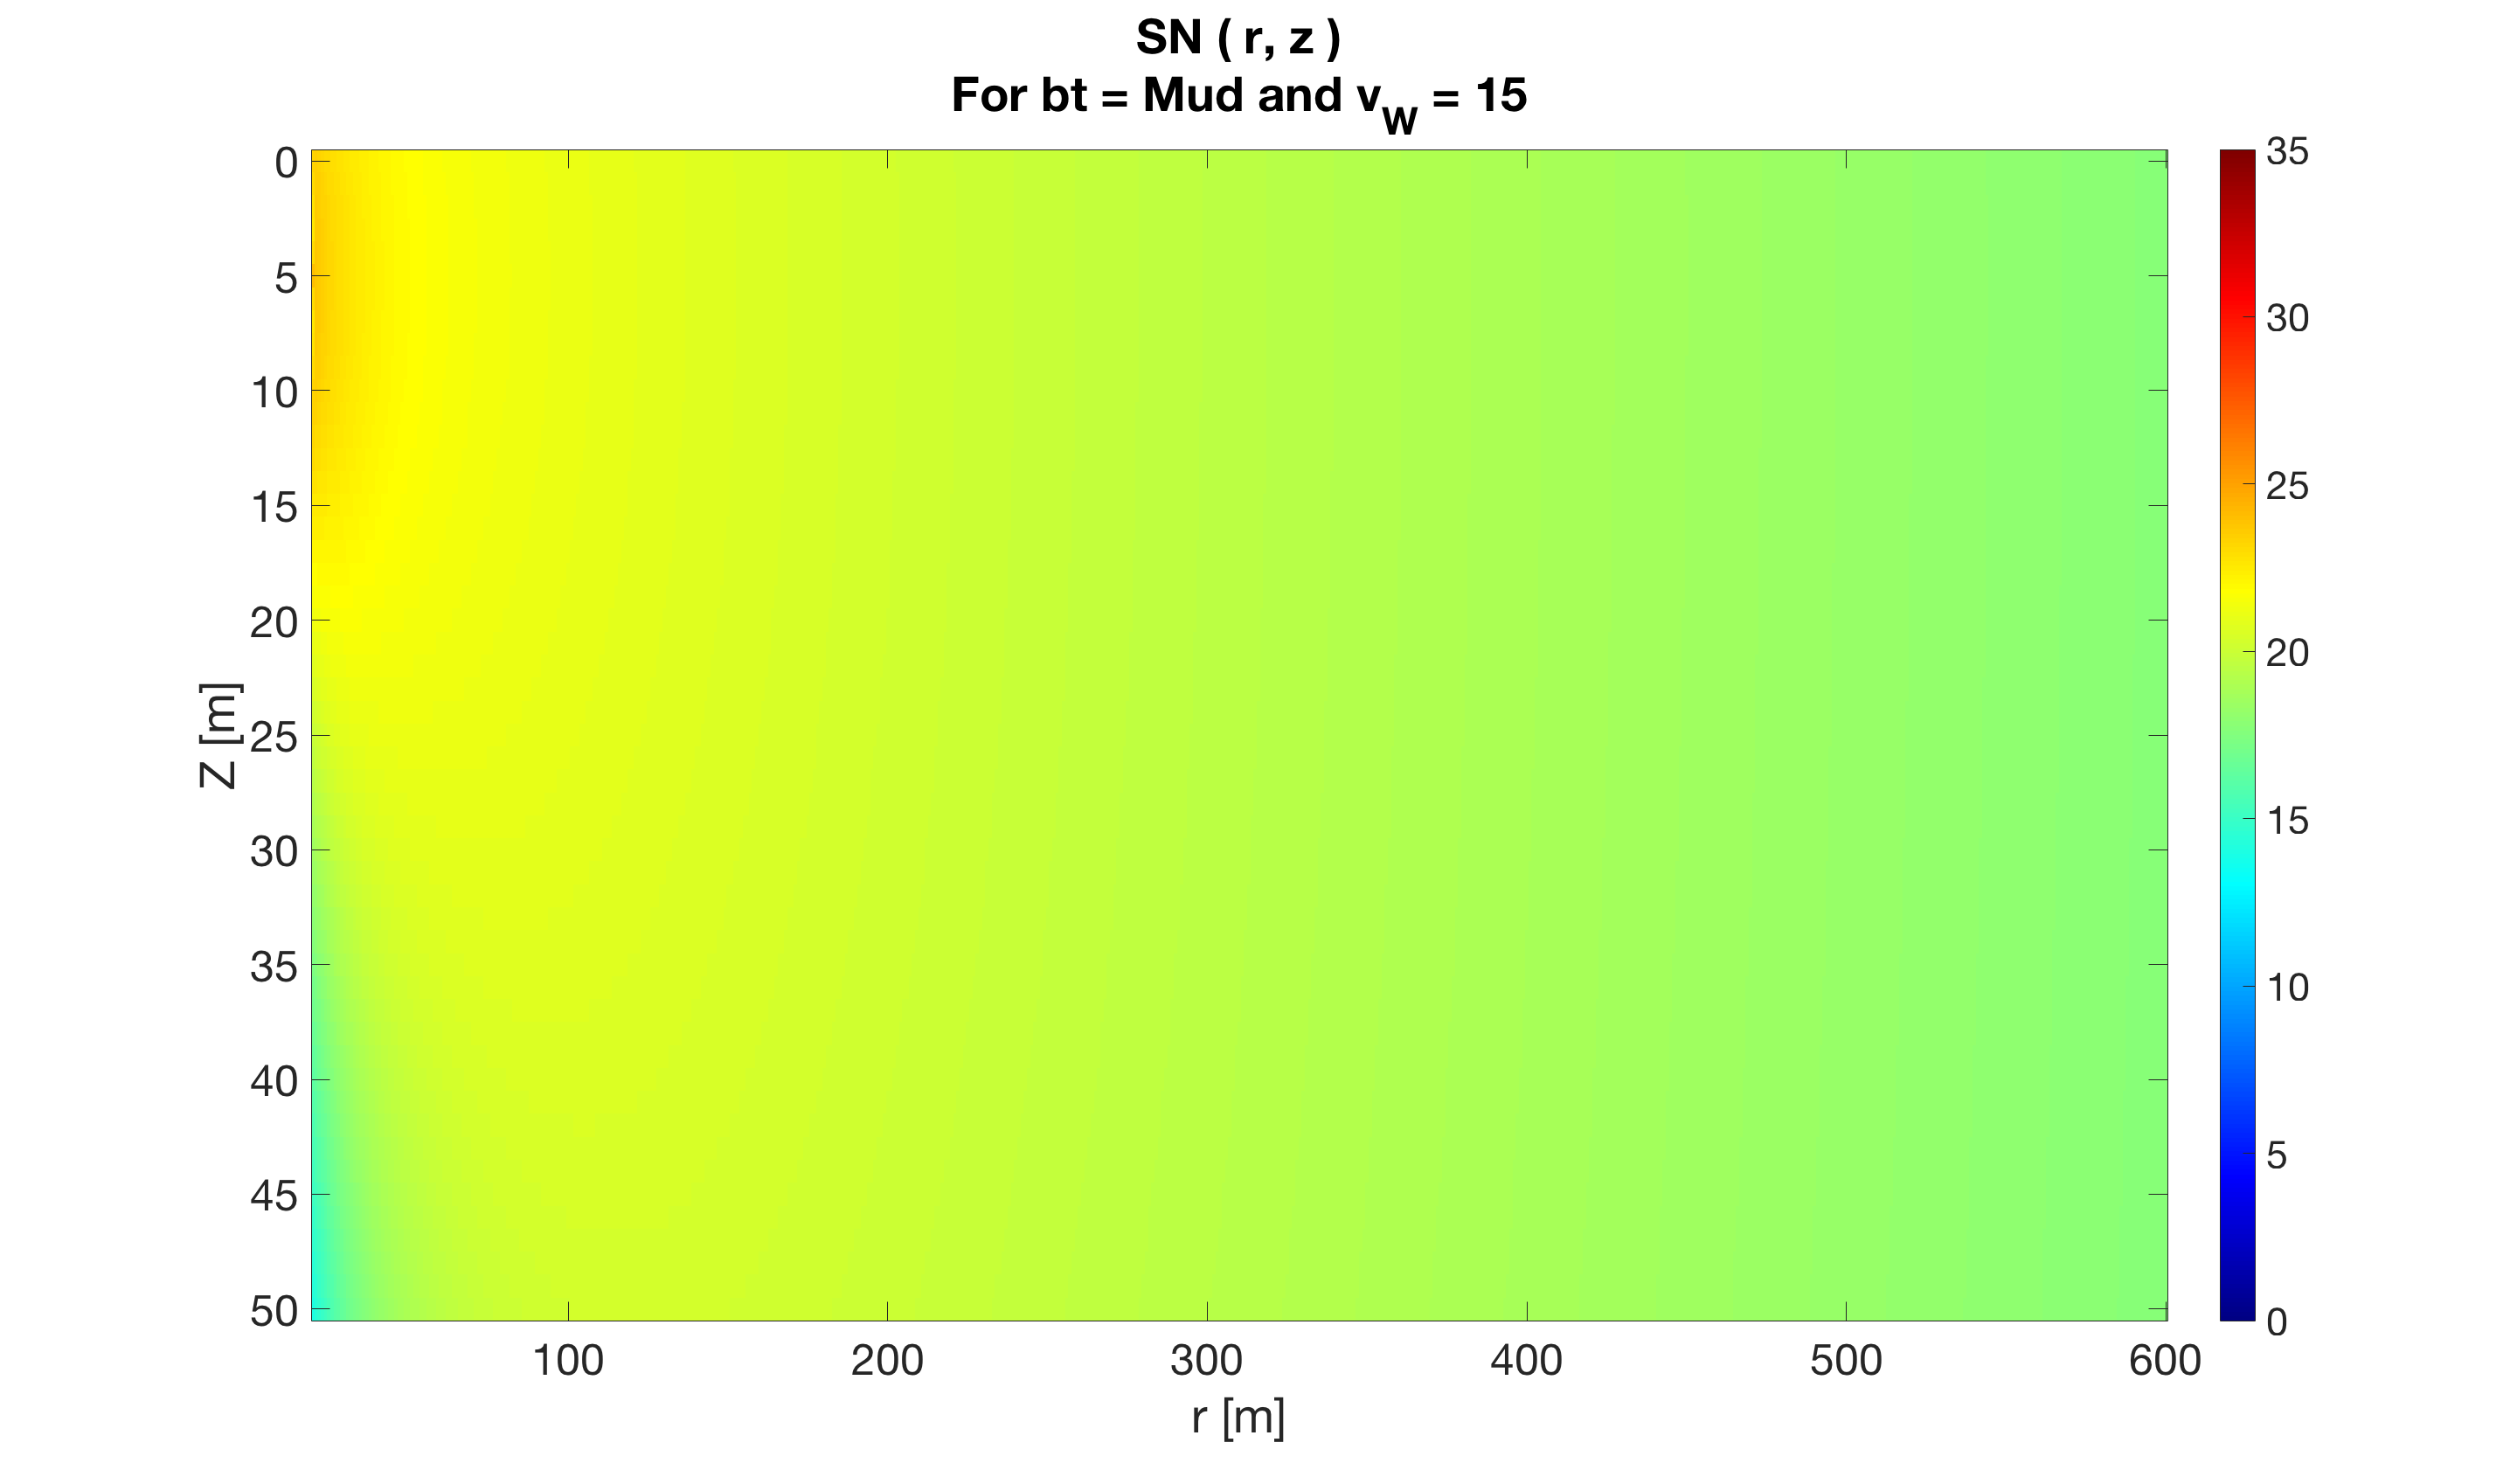
\includegraphics[width=95mm]{fig2.png}
}
\newline
\hbox to 18.5mm{}% !!
\subfloat[Wind speed = 25 kn]{
  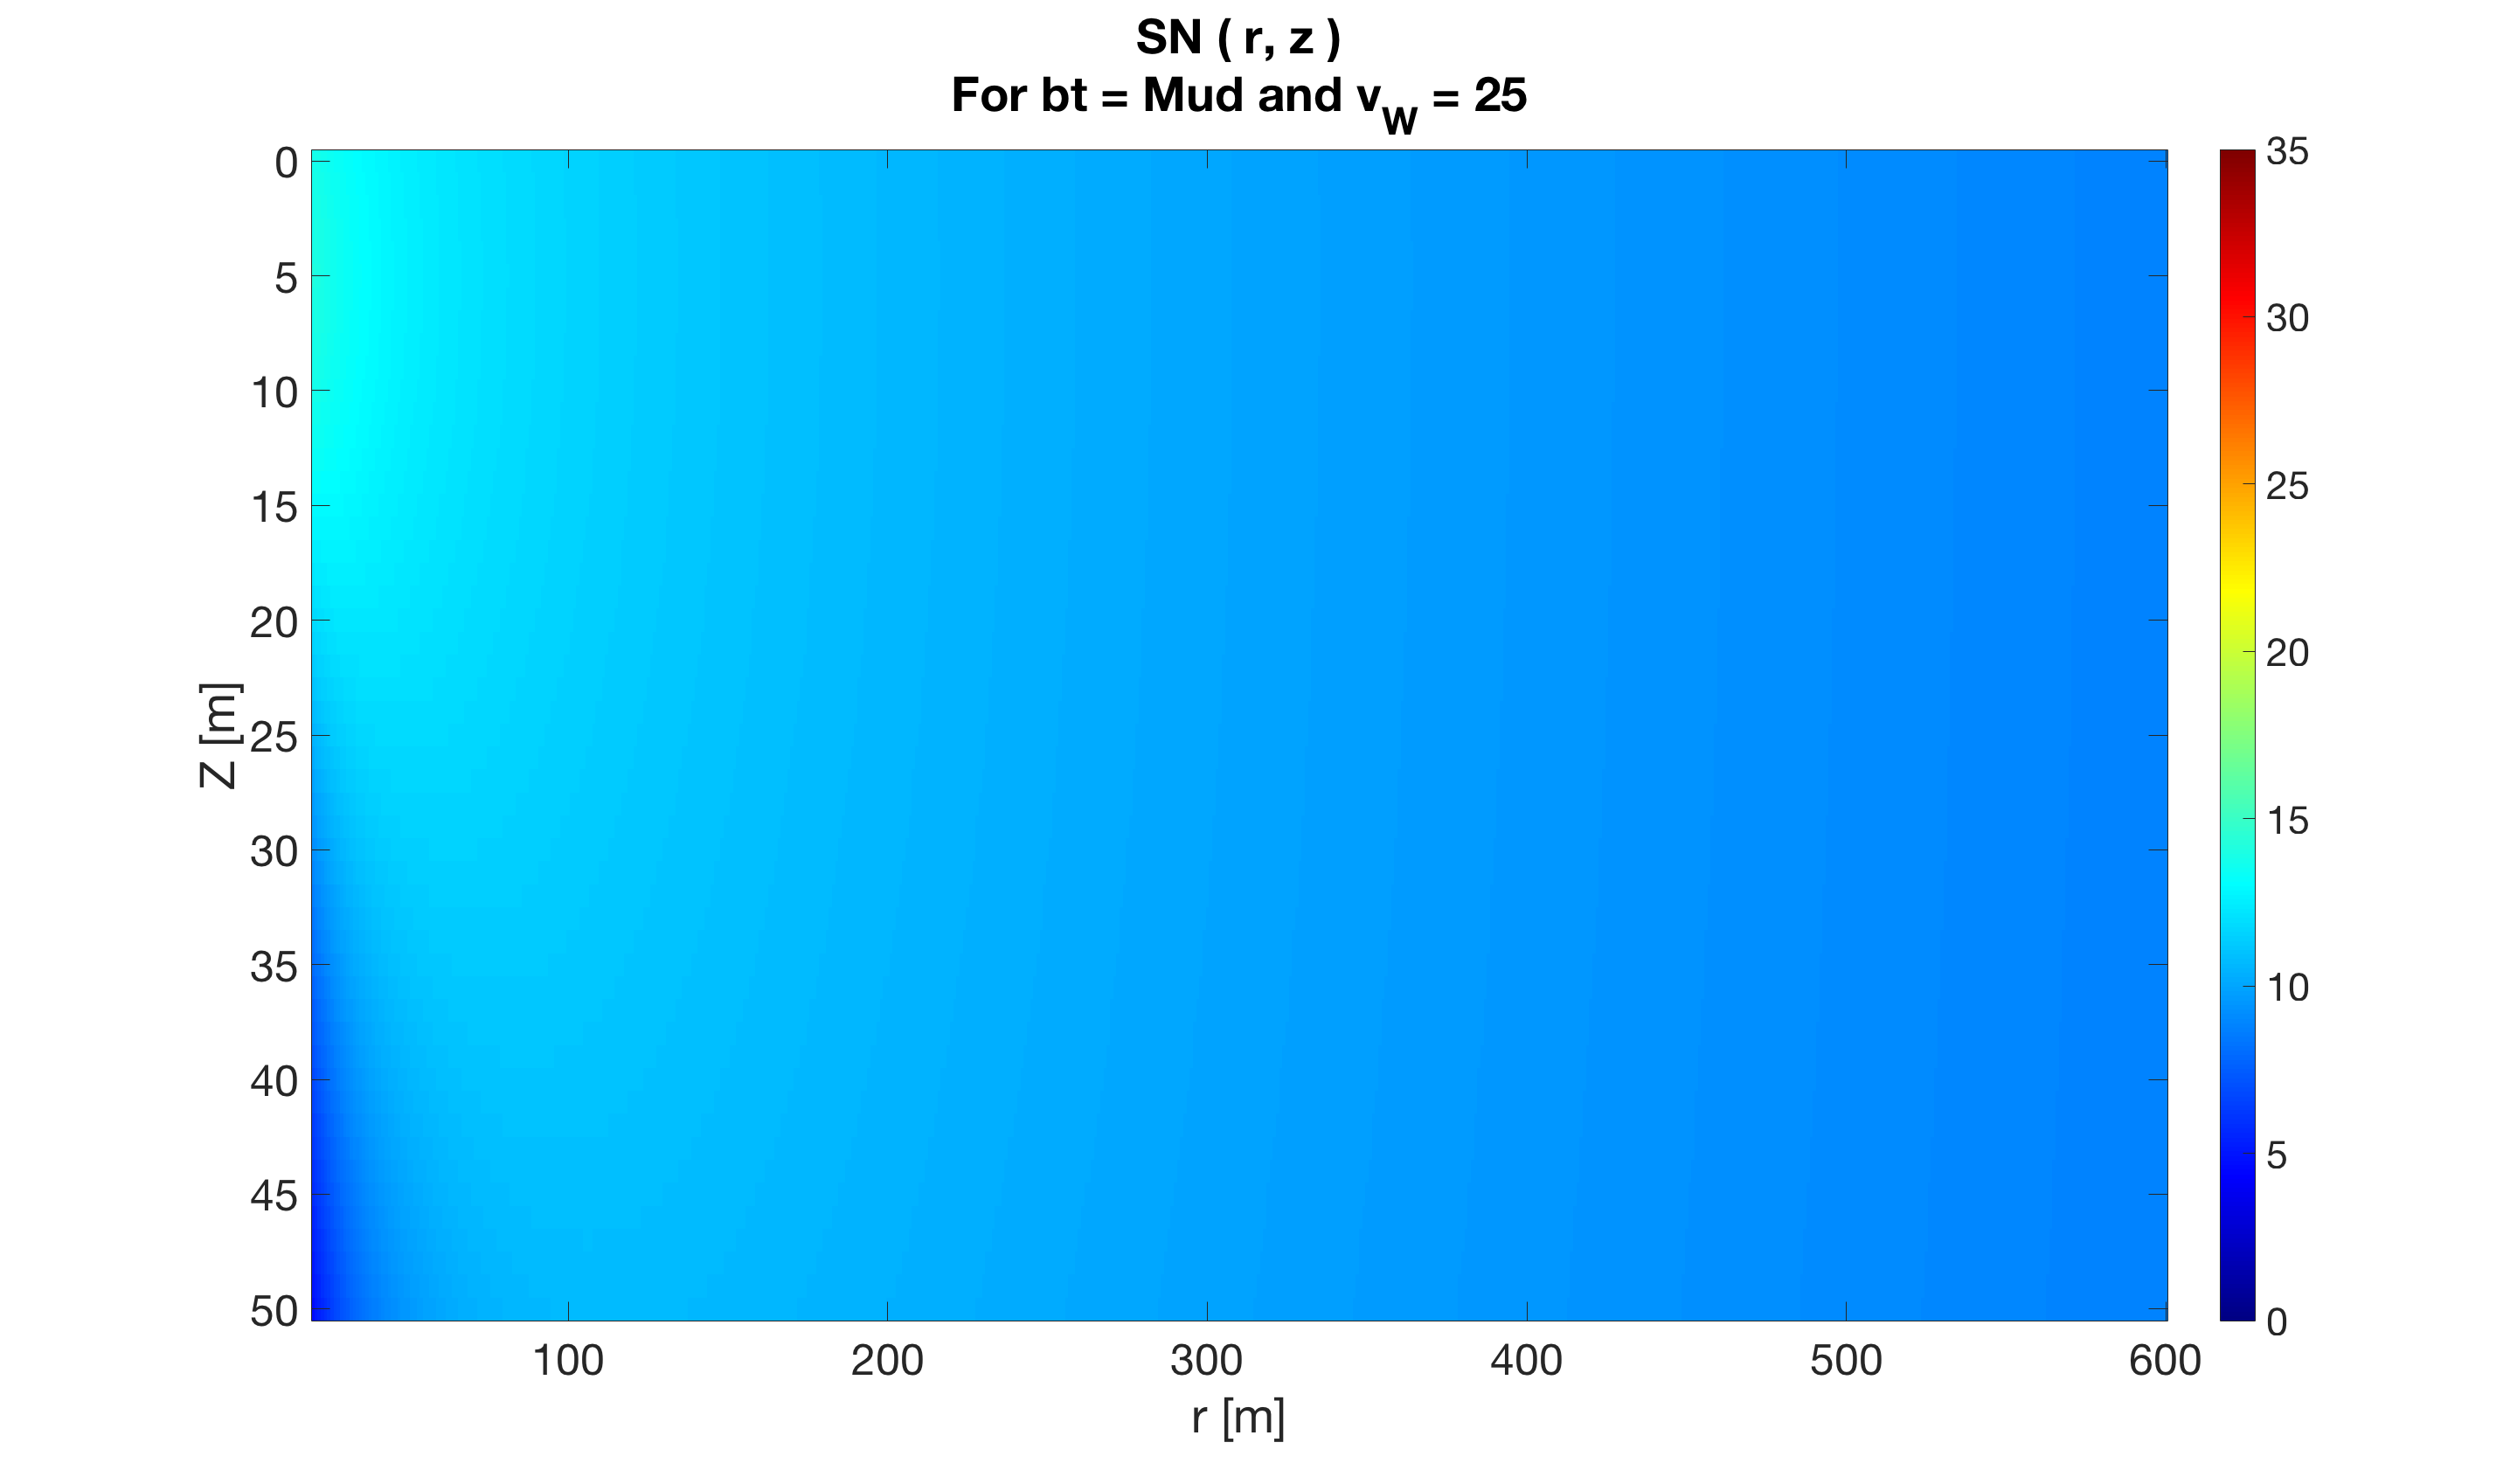
\includegraphics[width=95mm]{fig3.png}
}
\caption{Impact of mud as the bottom type and wind speed of 5, 15 and 25 knots on the signal to noise ratio}
\end{figure}

\noindent The Figure 1 shows the impact of wind speed on signal to noise ratio in the range of $\textit{r} (50, 600).$ The figure has been plotted for fixed value of wind speeds (5 kn, 15 kn and 25 kn) and the bottom type is considered to be mud. We can see from the Figure 1 that as the wind speed is increased from 5 kn to 25 kn, the signal to noise ratio decreases.

\begin{figure}[h]
\centering
\subfloat[third]{
  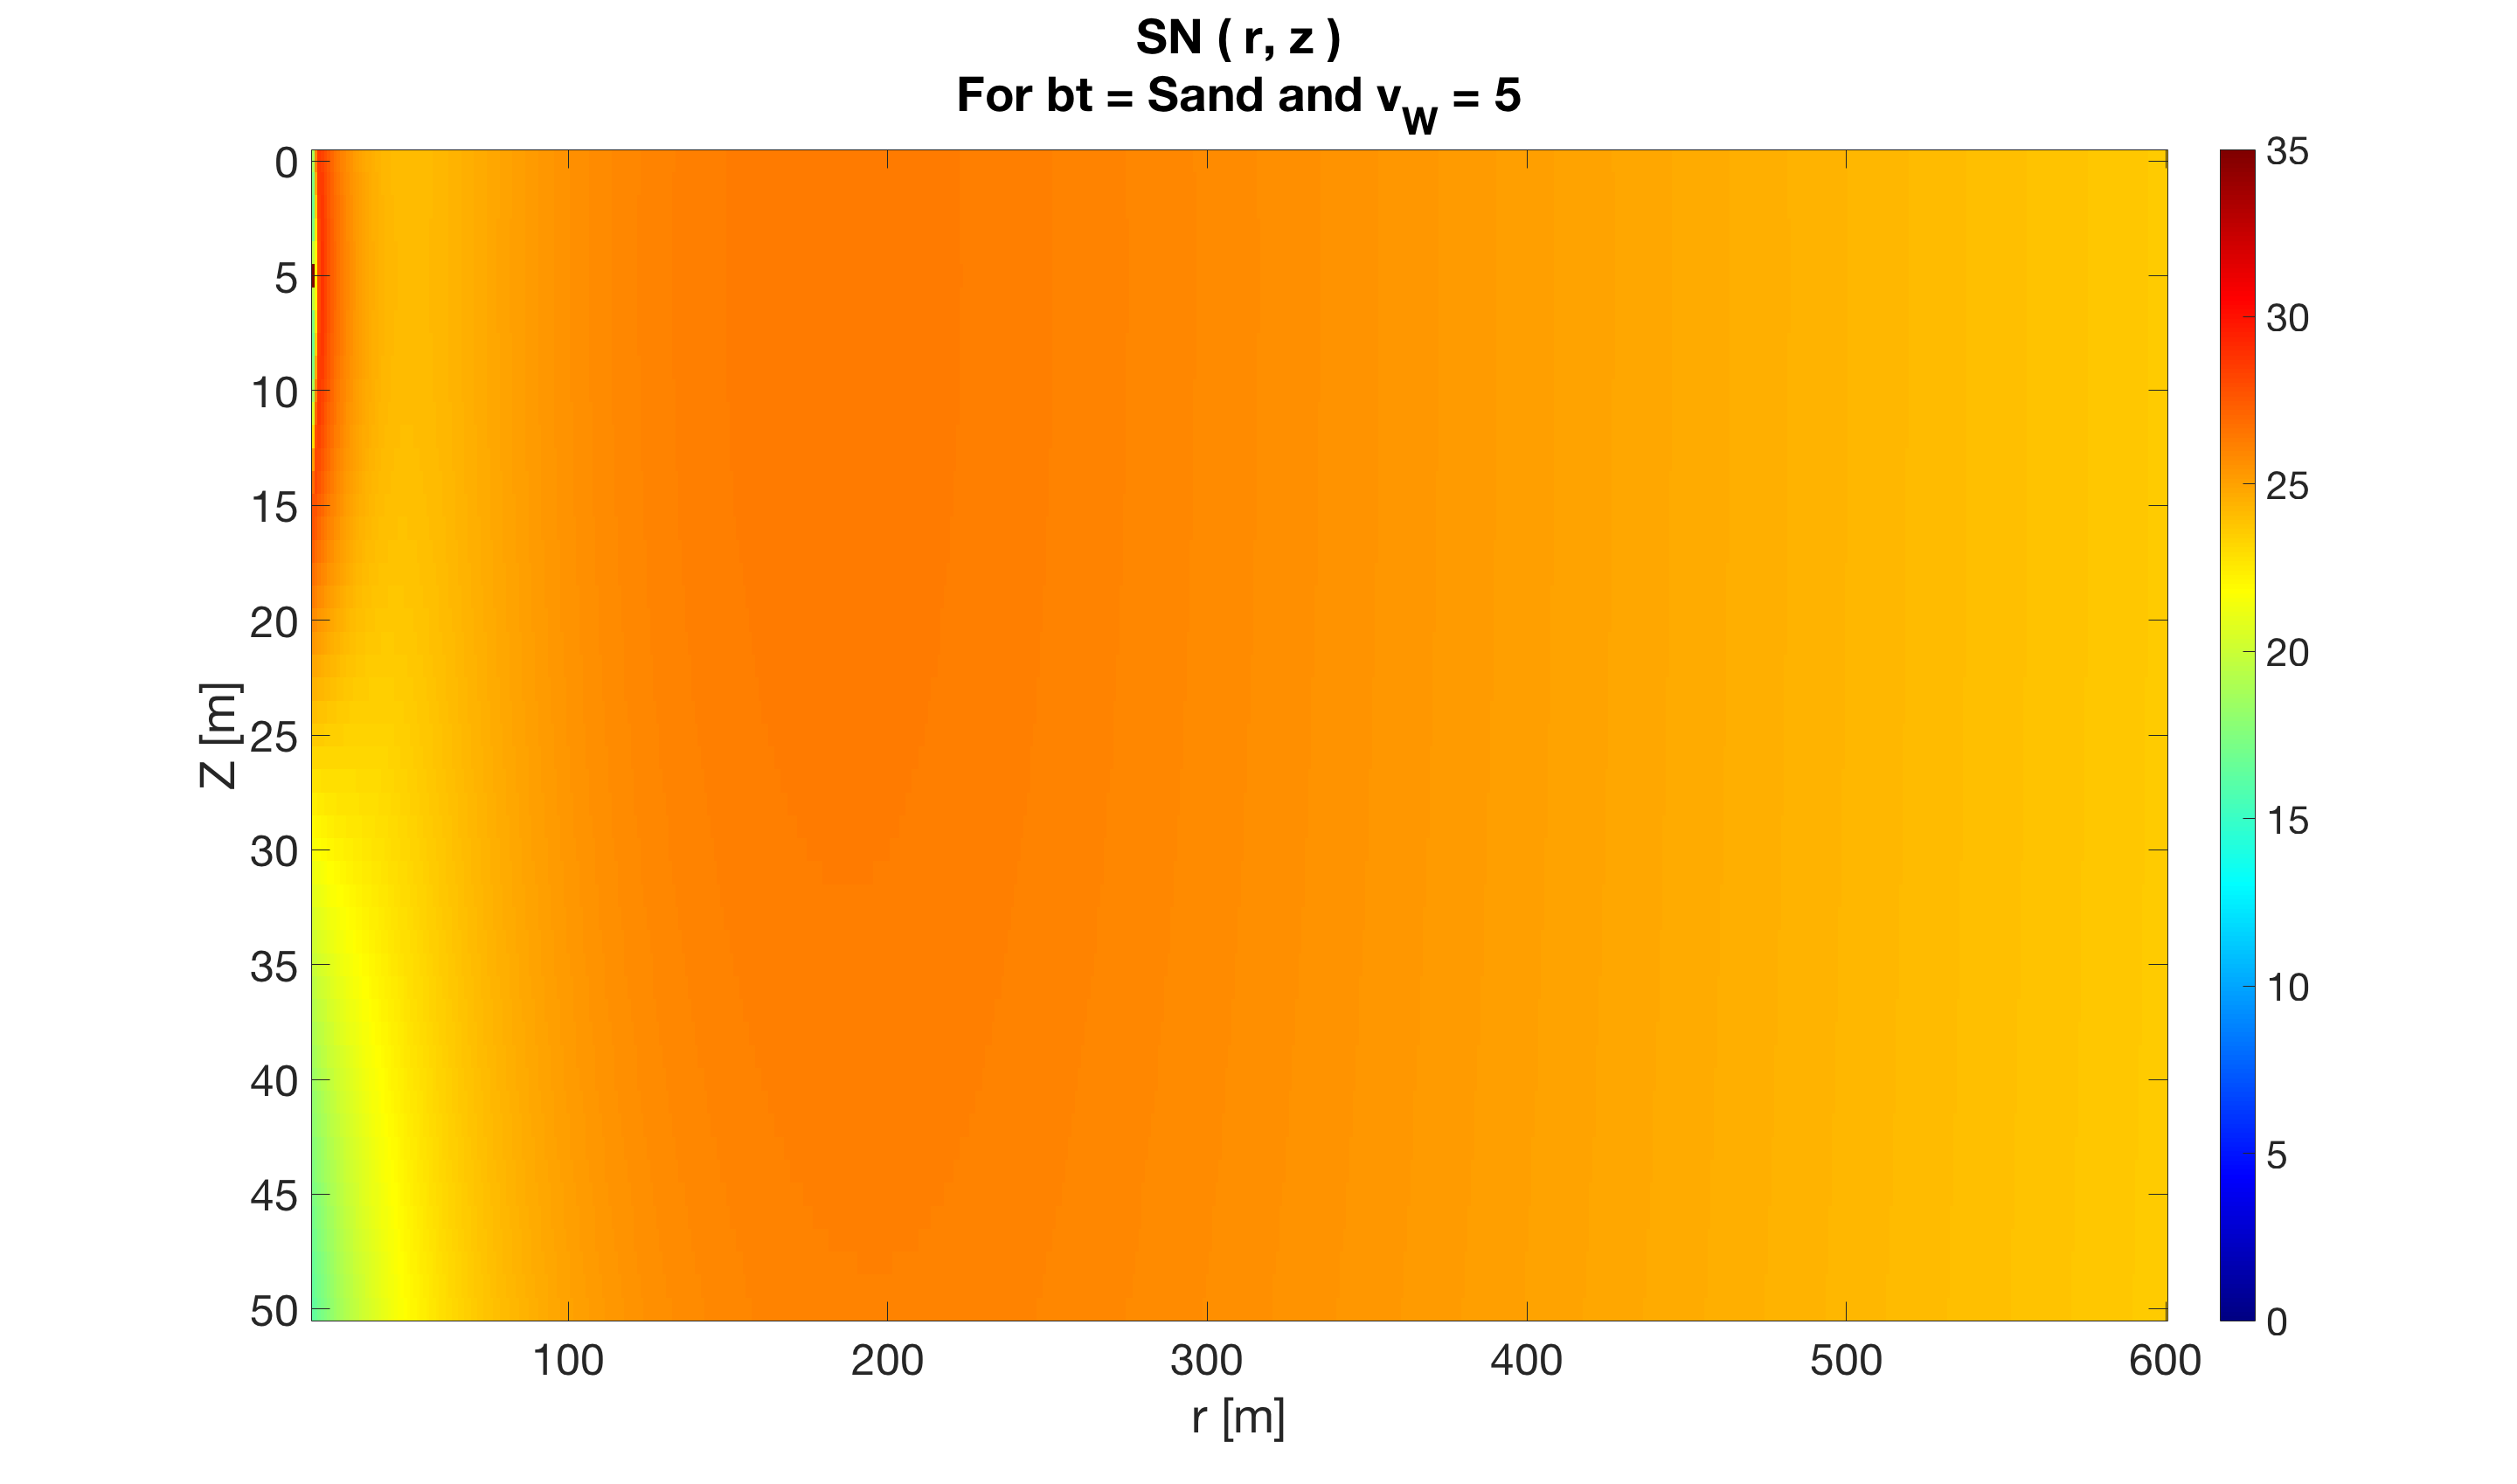
\includegraphics[width=95mm]{fig4.png}
}
\subfloat[forth]{
  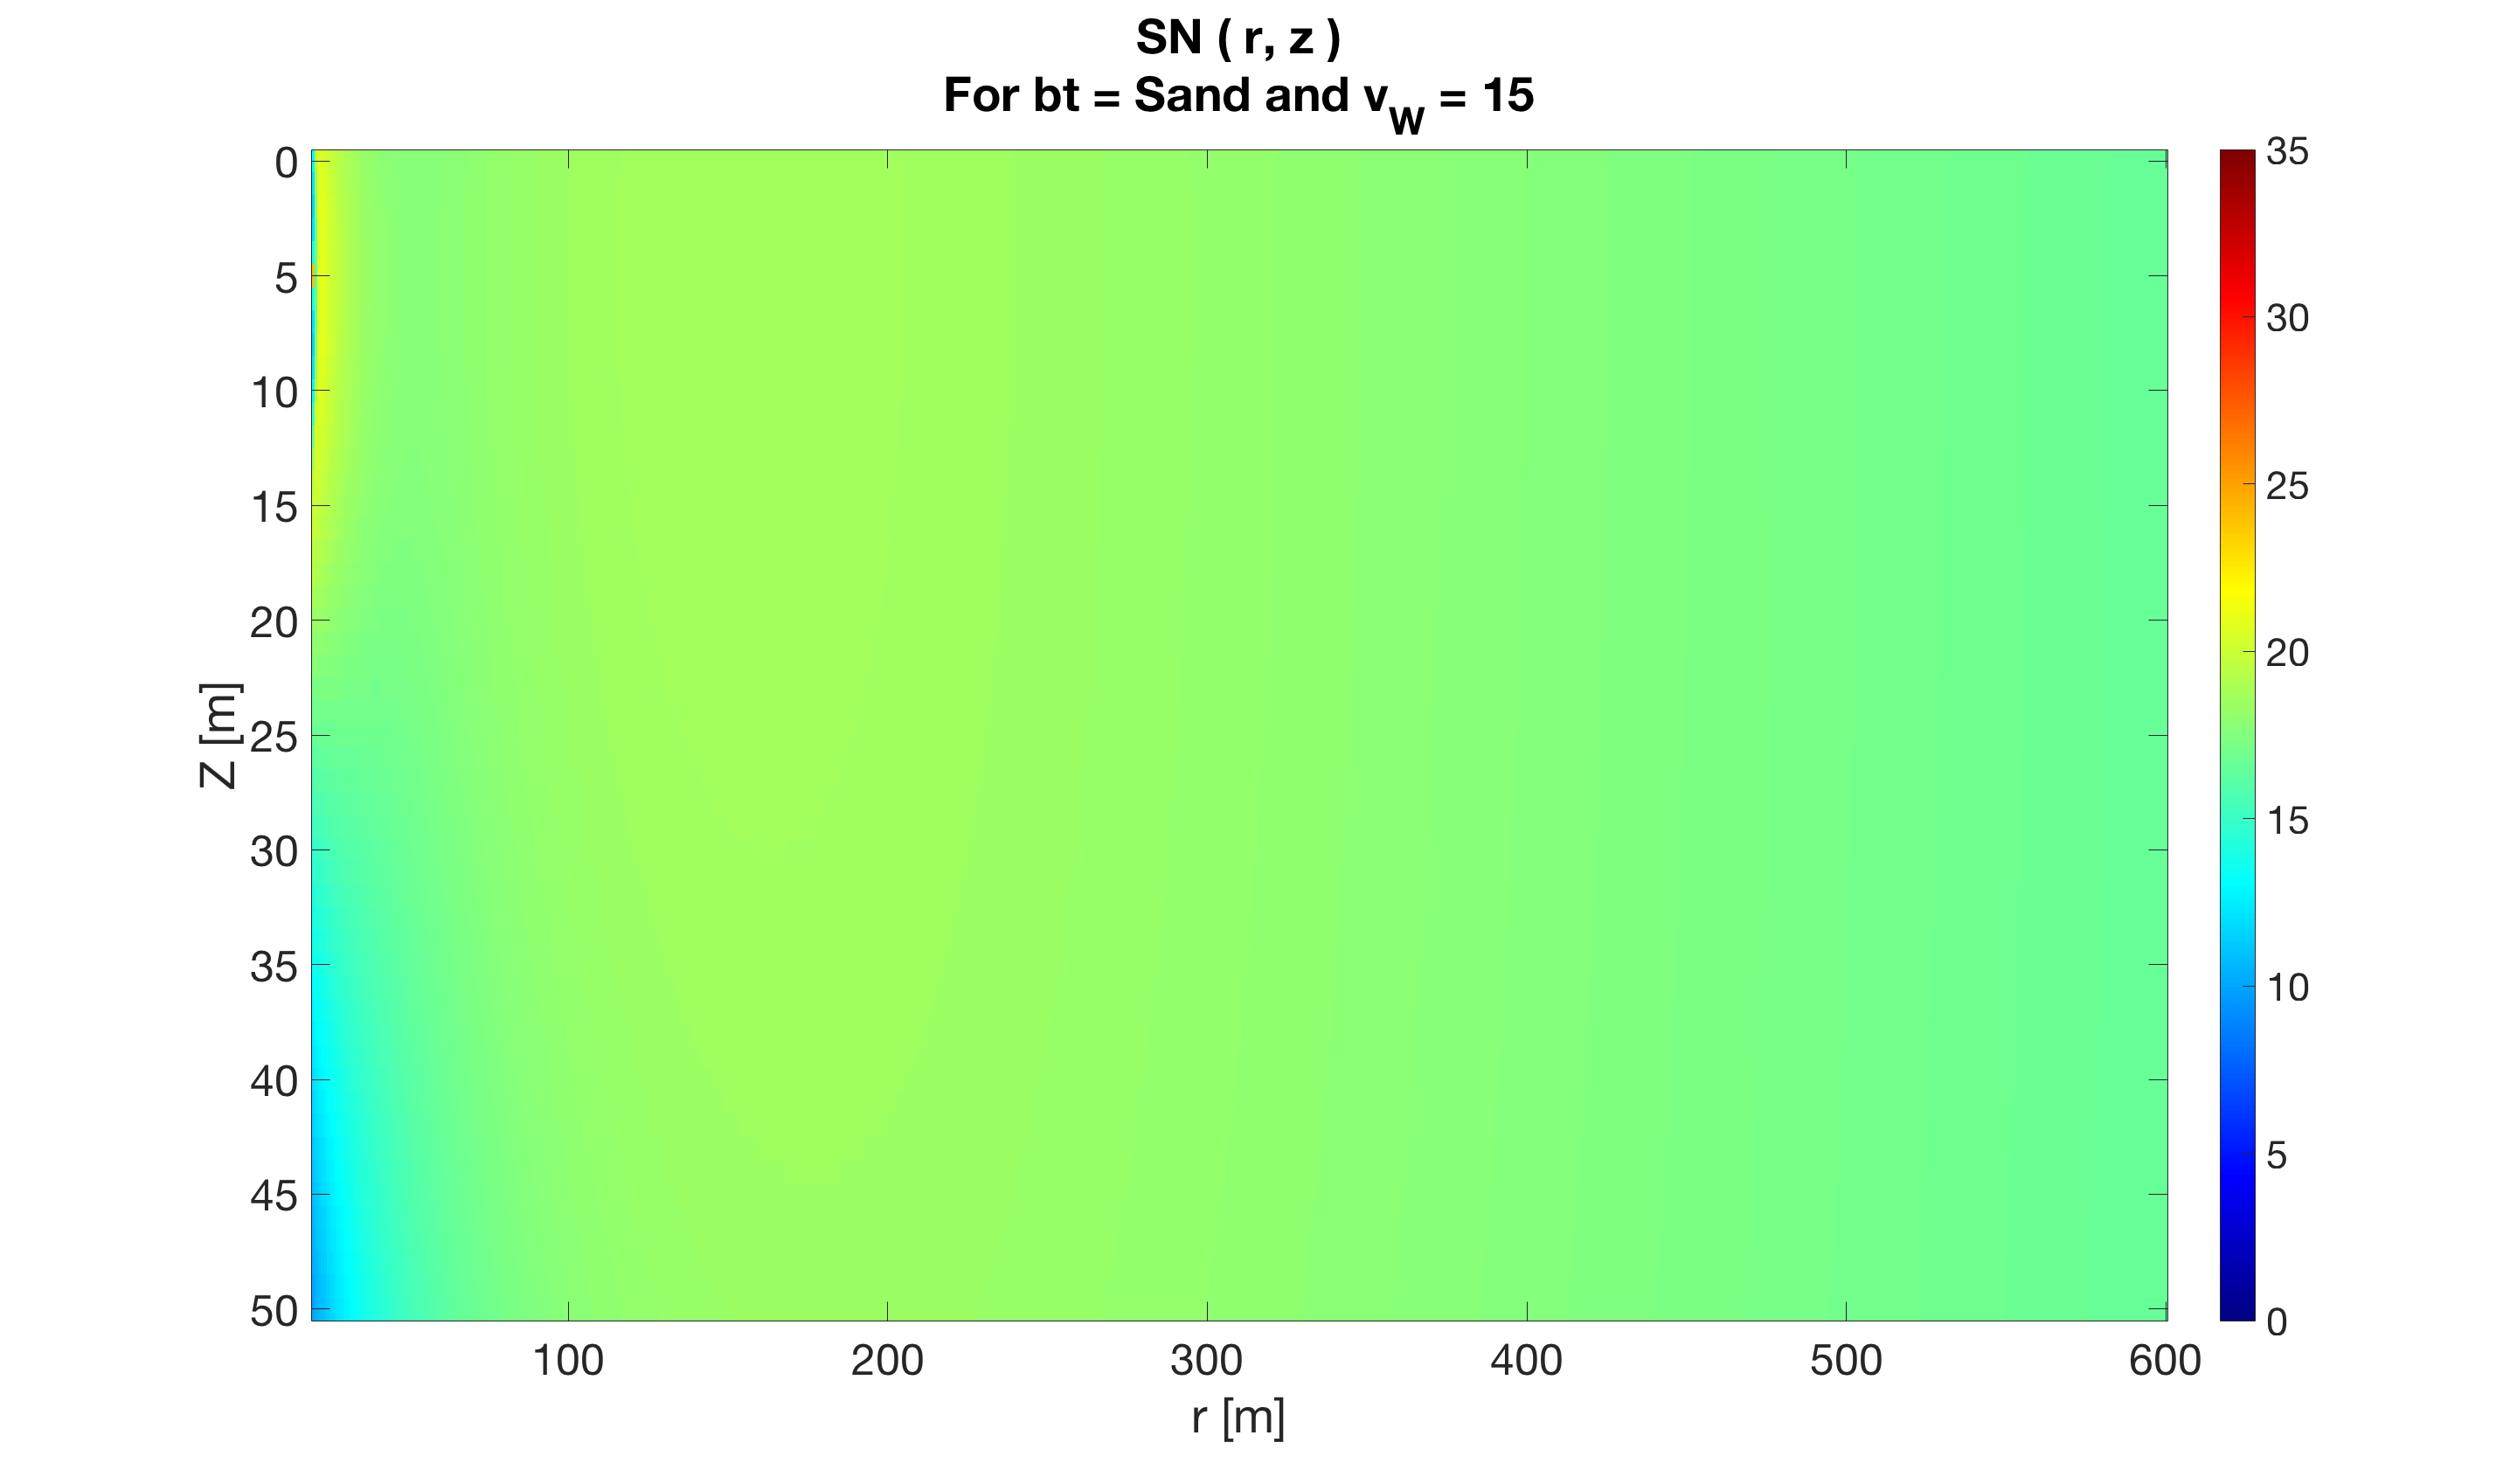
\includegraphics[width=95mm]{fig5.png}
}
\newline
\hbox to 18.5mm{}% !!
\subfloat[fifth]{
  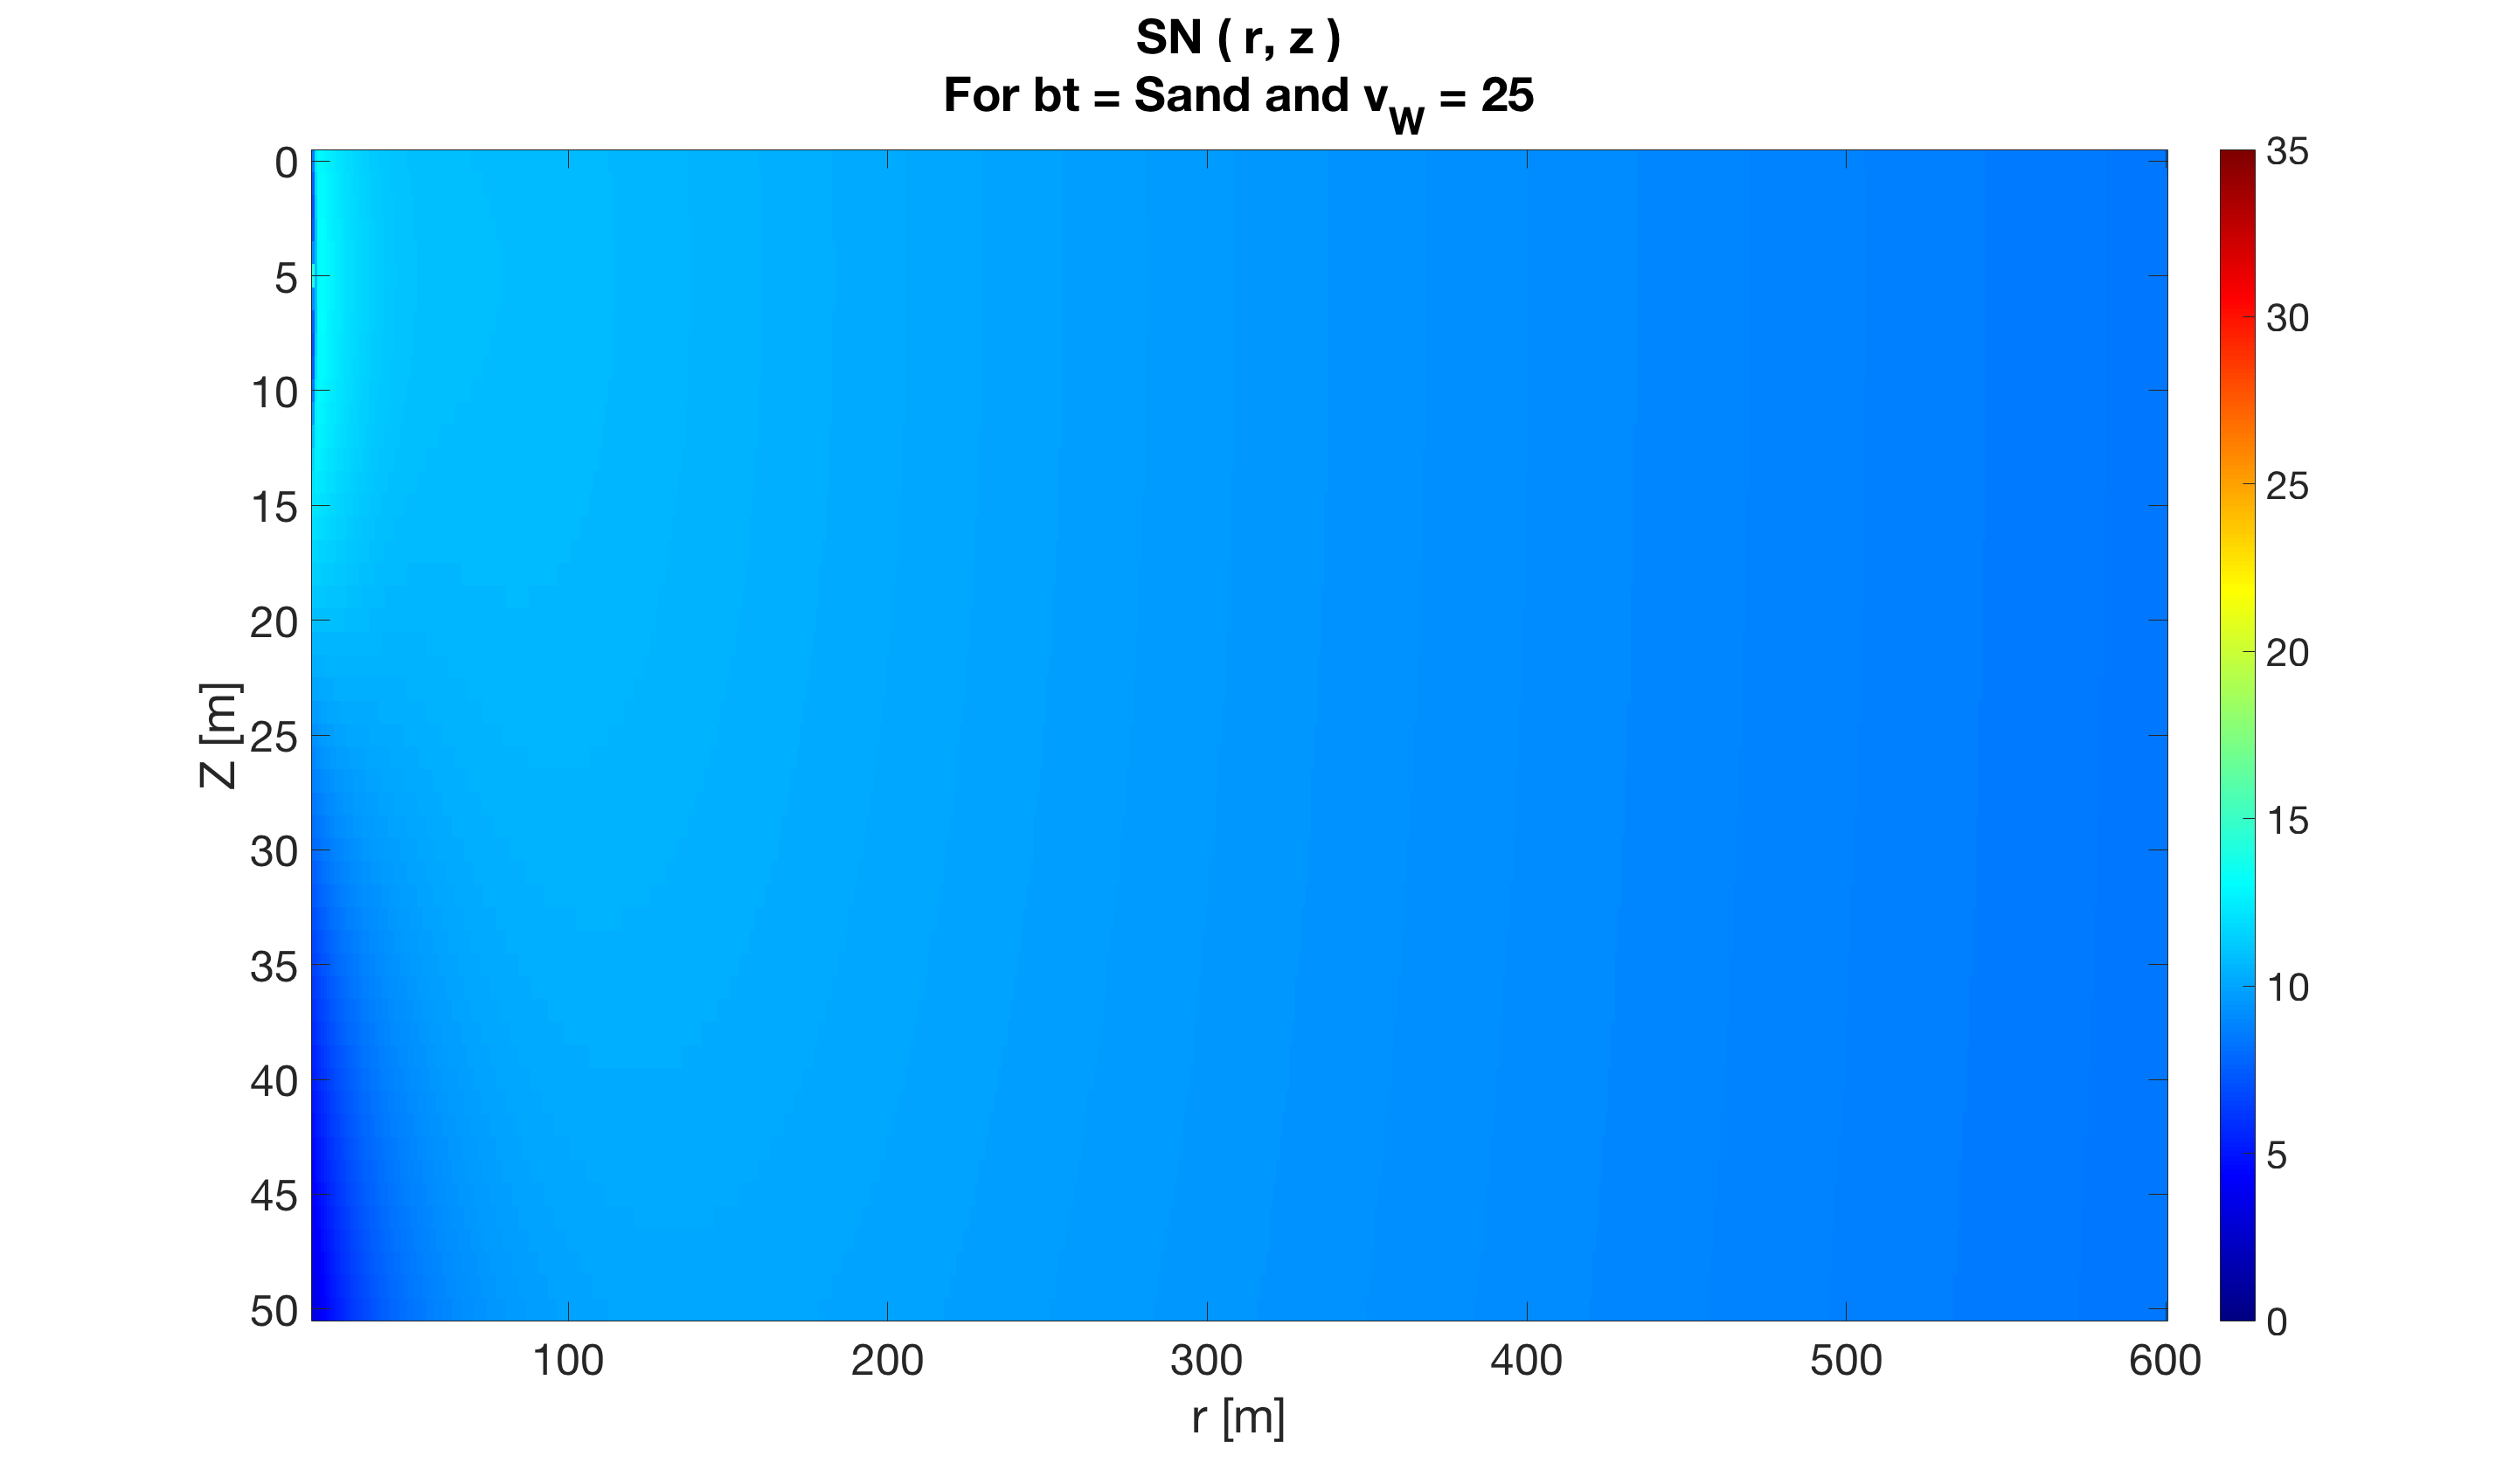
\includegraphics[width=90mm]{fig6.png}
}
\caption{Impact of sand as the bottom type and wind speed of 5, 15 and 25 knots on the signal to noise ratio}
\end{figure}

\noindent The figure 2 consists of plots with their bottom type as sand. When we compare Figure 2 to Figure 1, we noticed that the signal to noise ratio (SNR) is decreased as the bottom type changed from mud to sand. Also, the dependence if wind speed is similar to that of Figure 1. 

\newpage

\begin{figure}[h]
\centering
\subfloat[first]{
  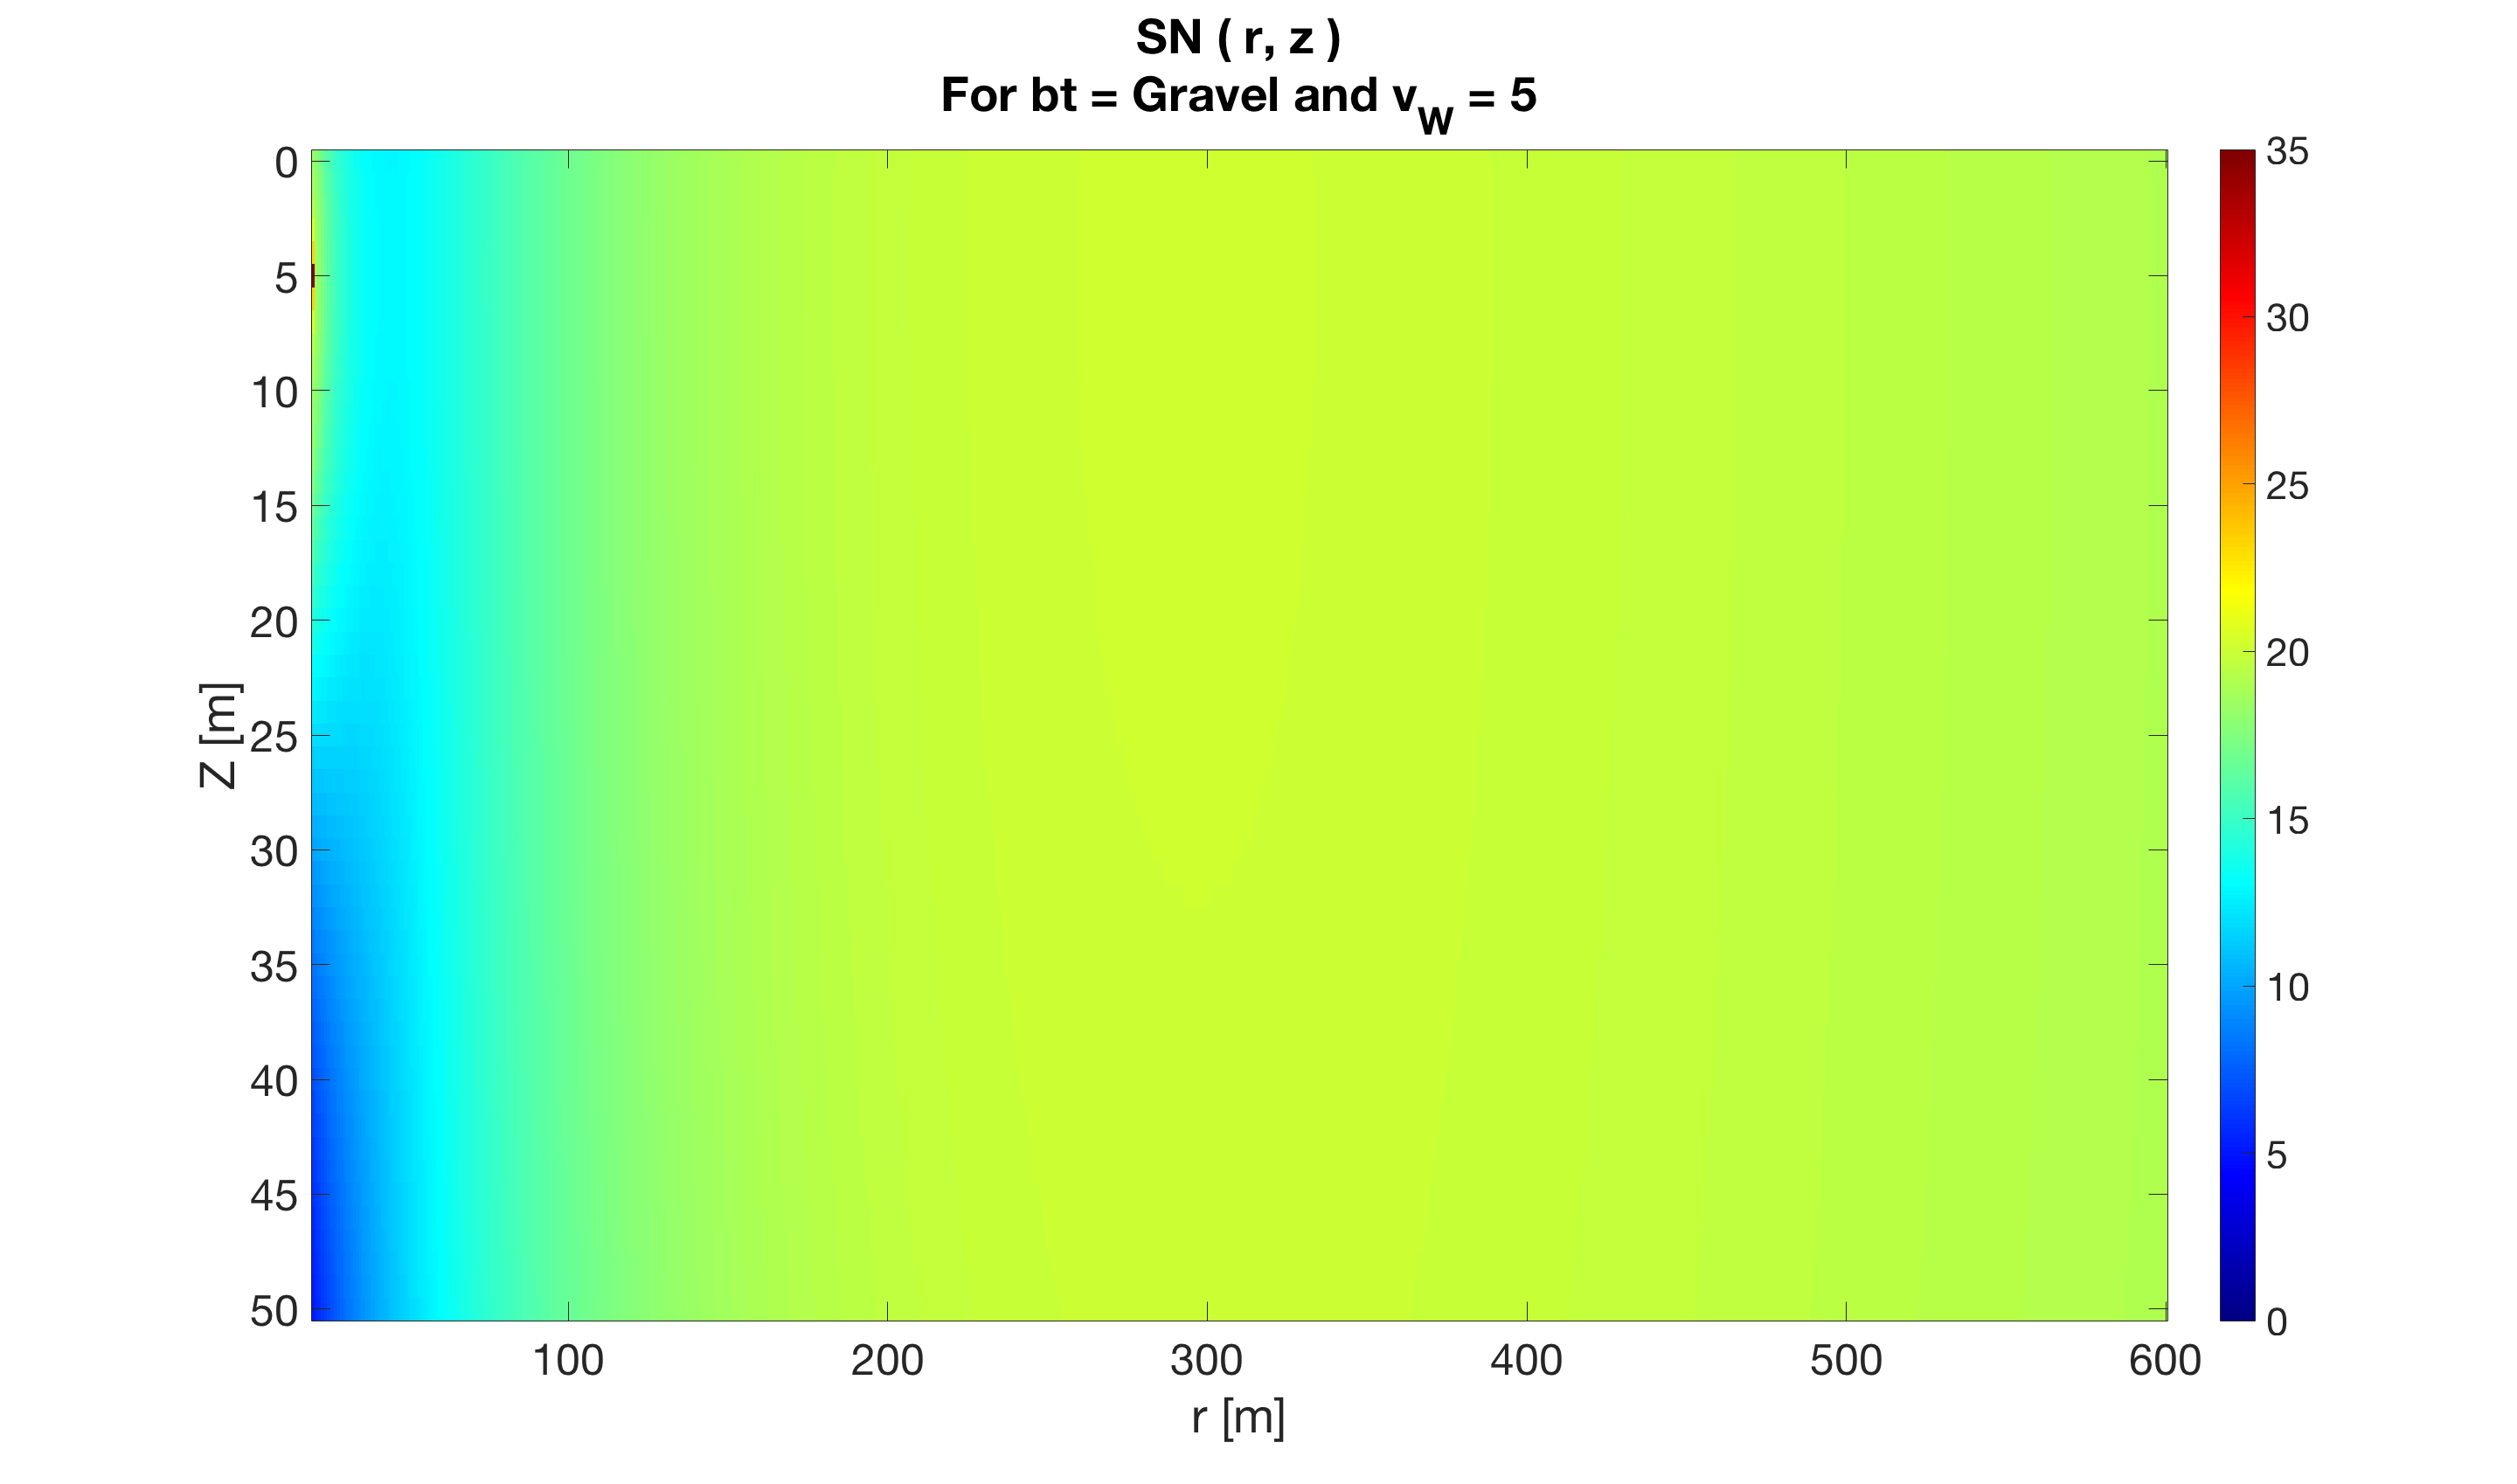
\includegraphics[width=95mm]{fig7.png}
}
\subfloat[second]{
  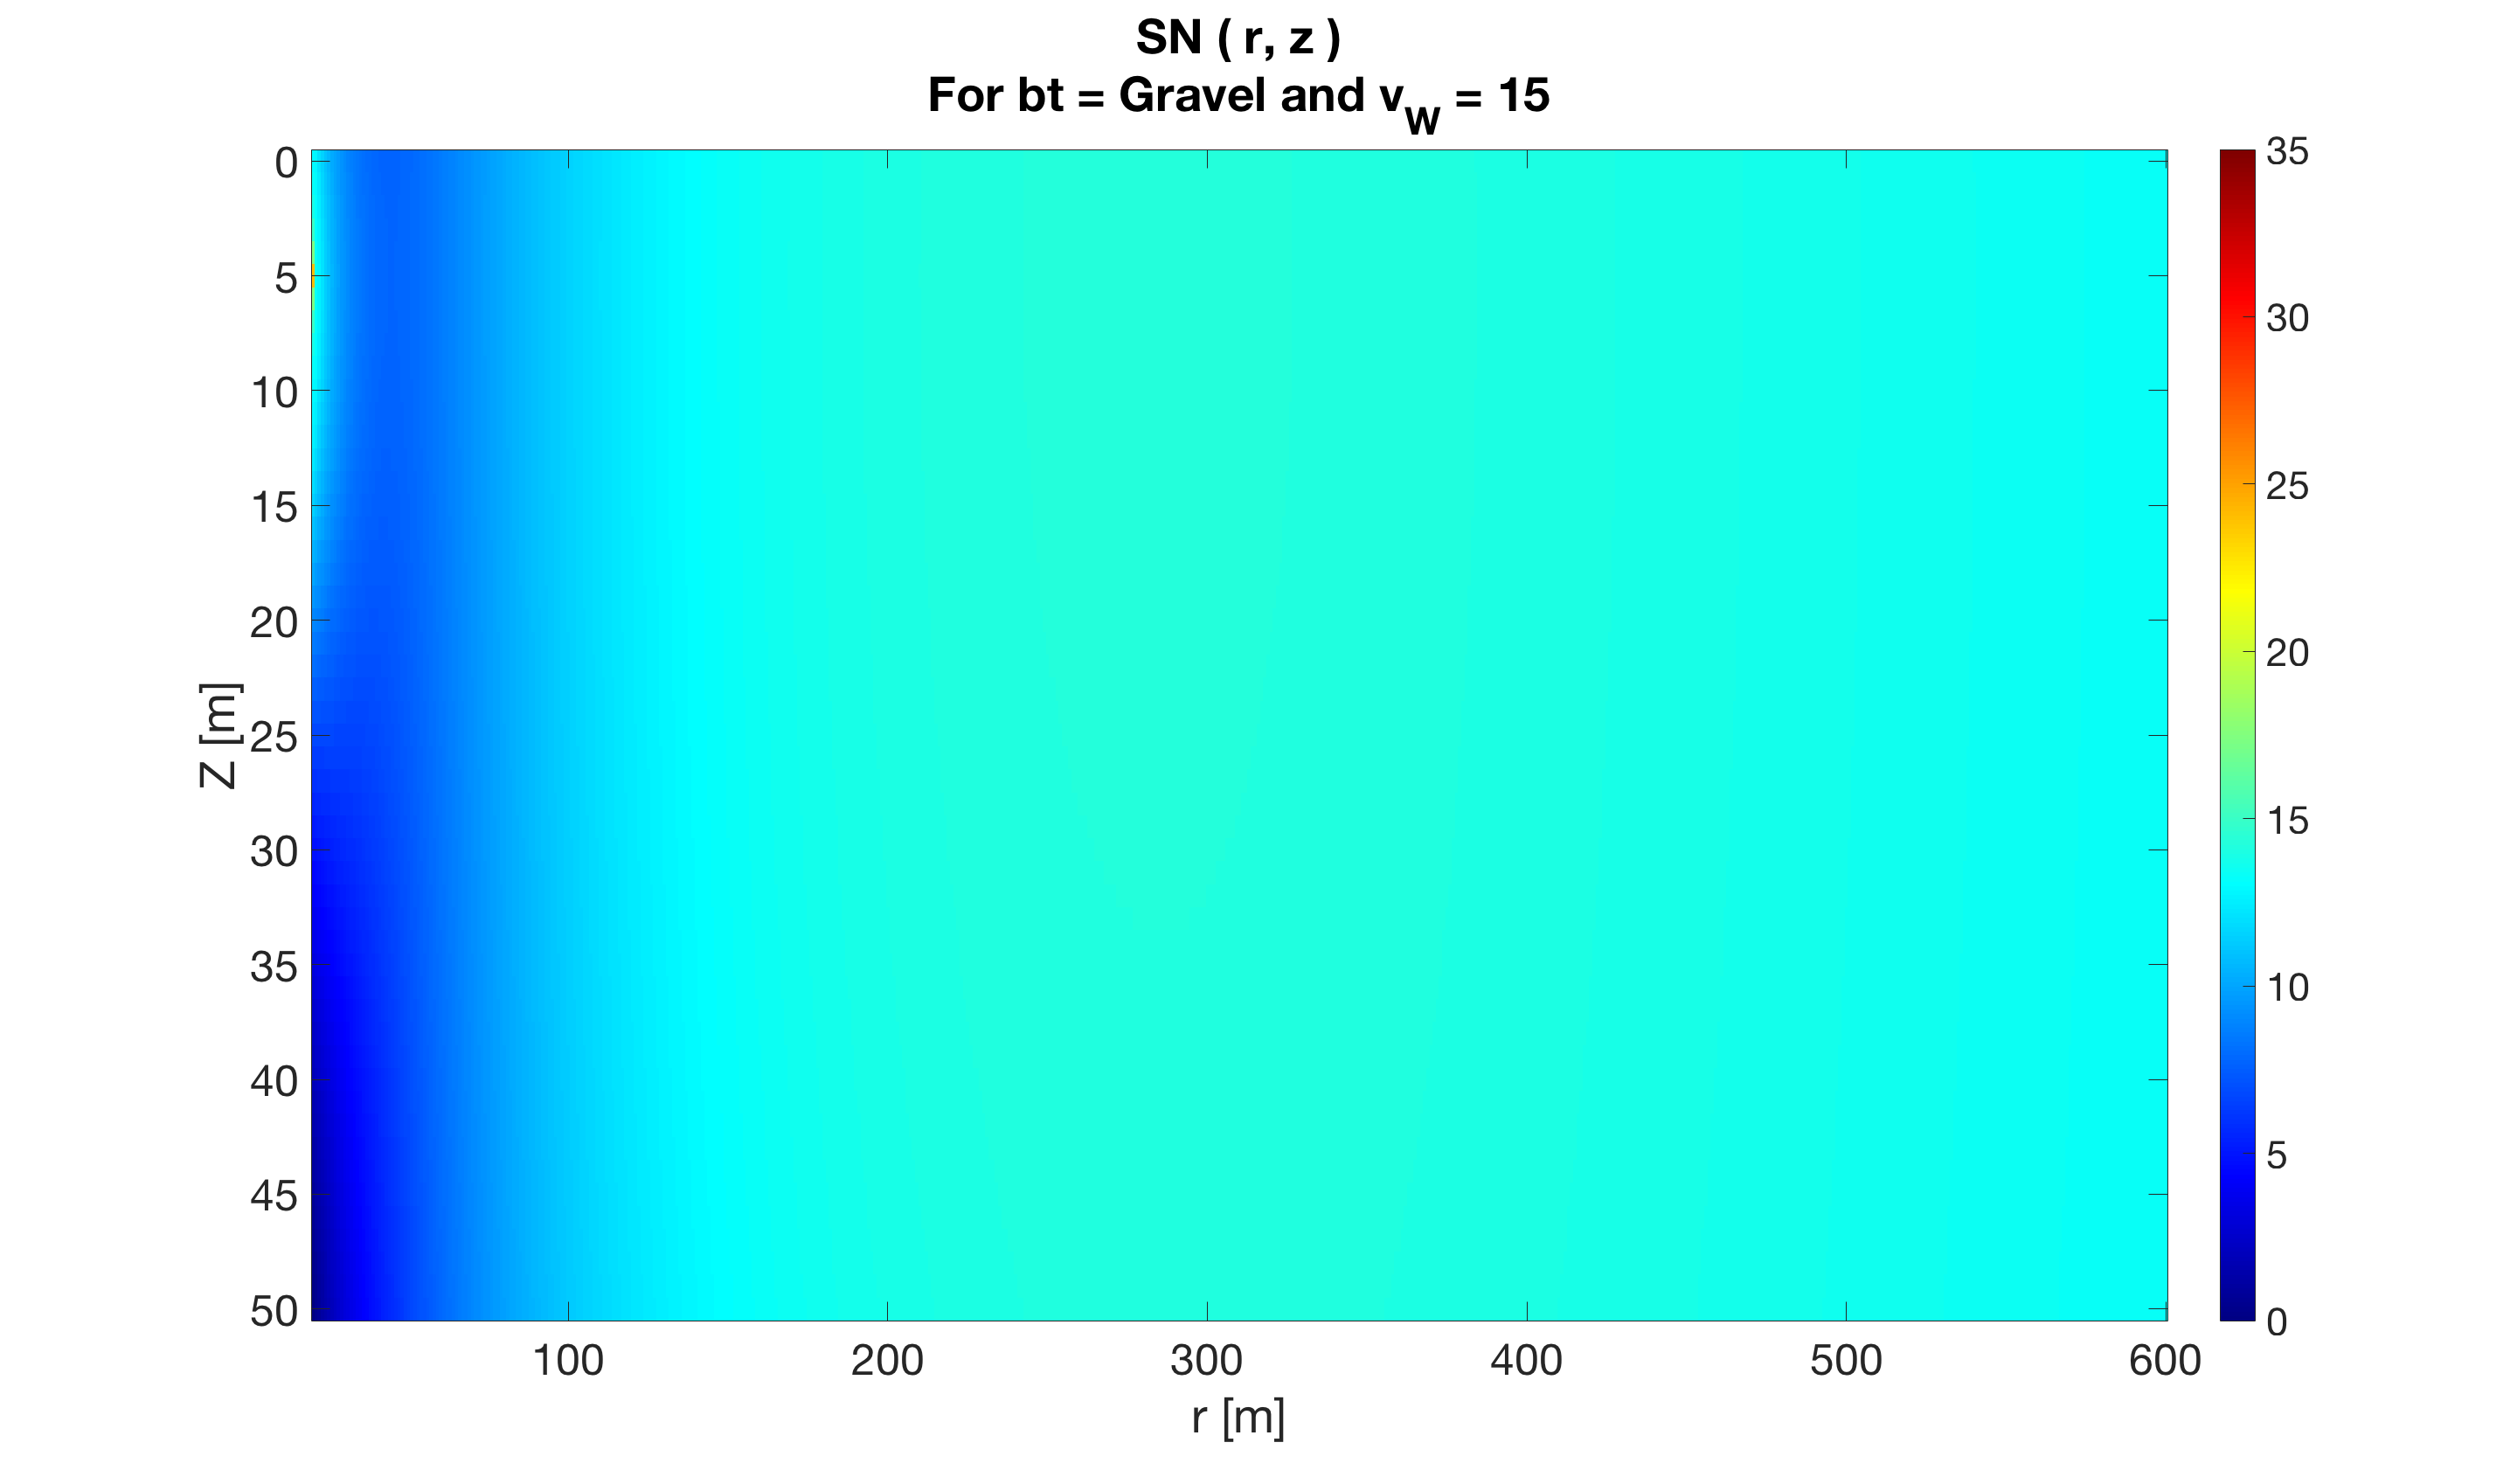
\includegraphics[width=95mm]{fig8.png}
}
\newline
\hbox to 18.5mm{}% !!
\subfloat[fifth]{
  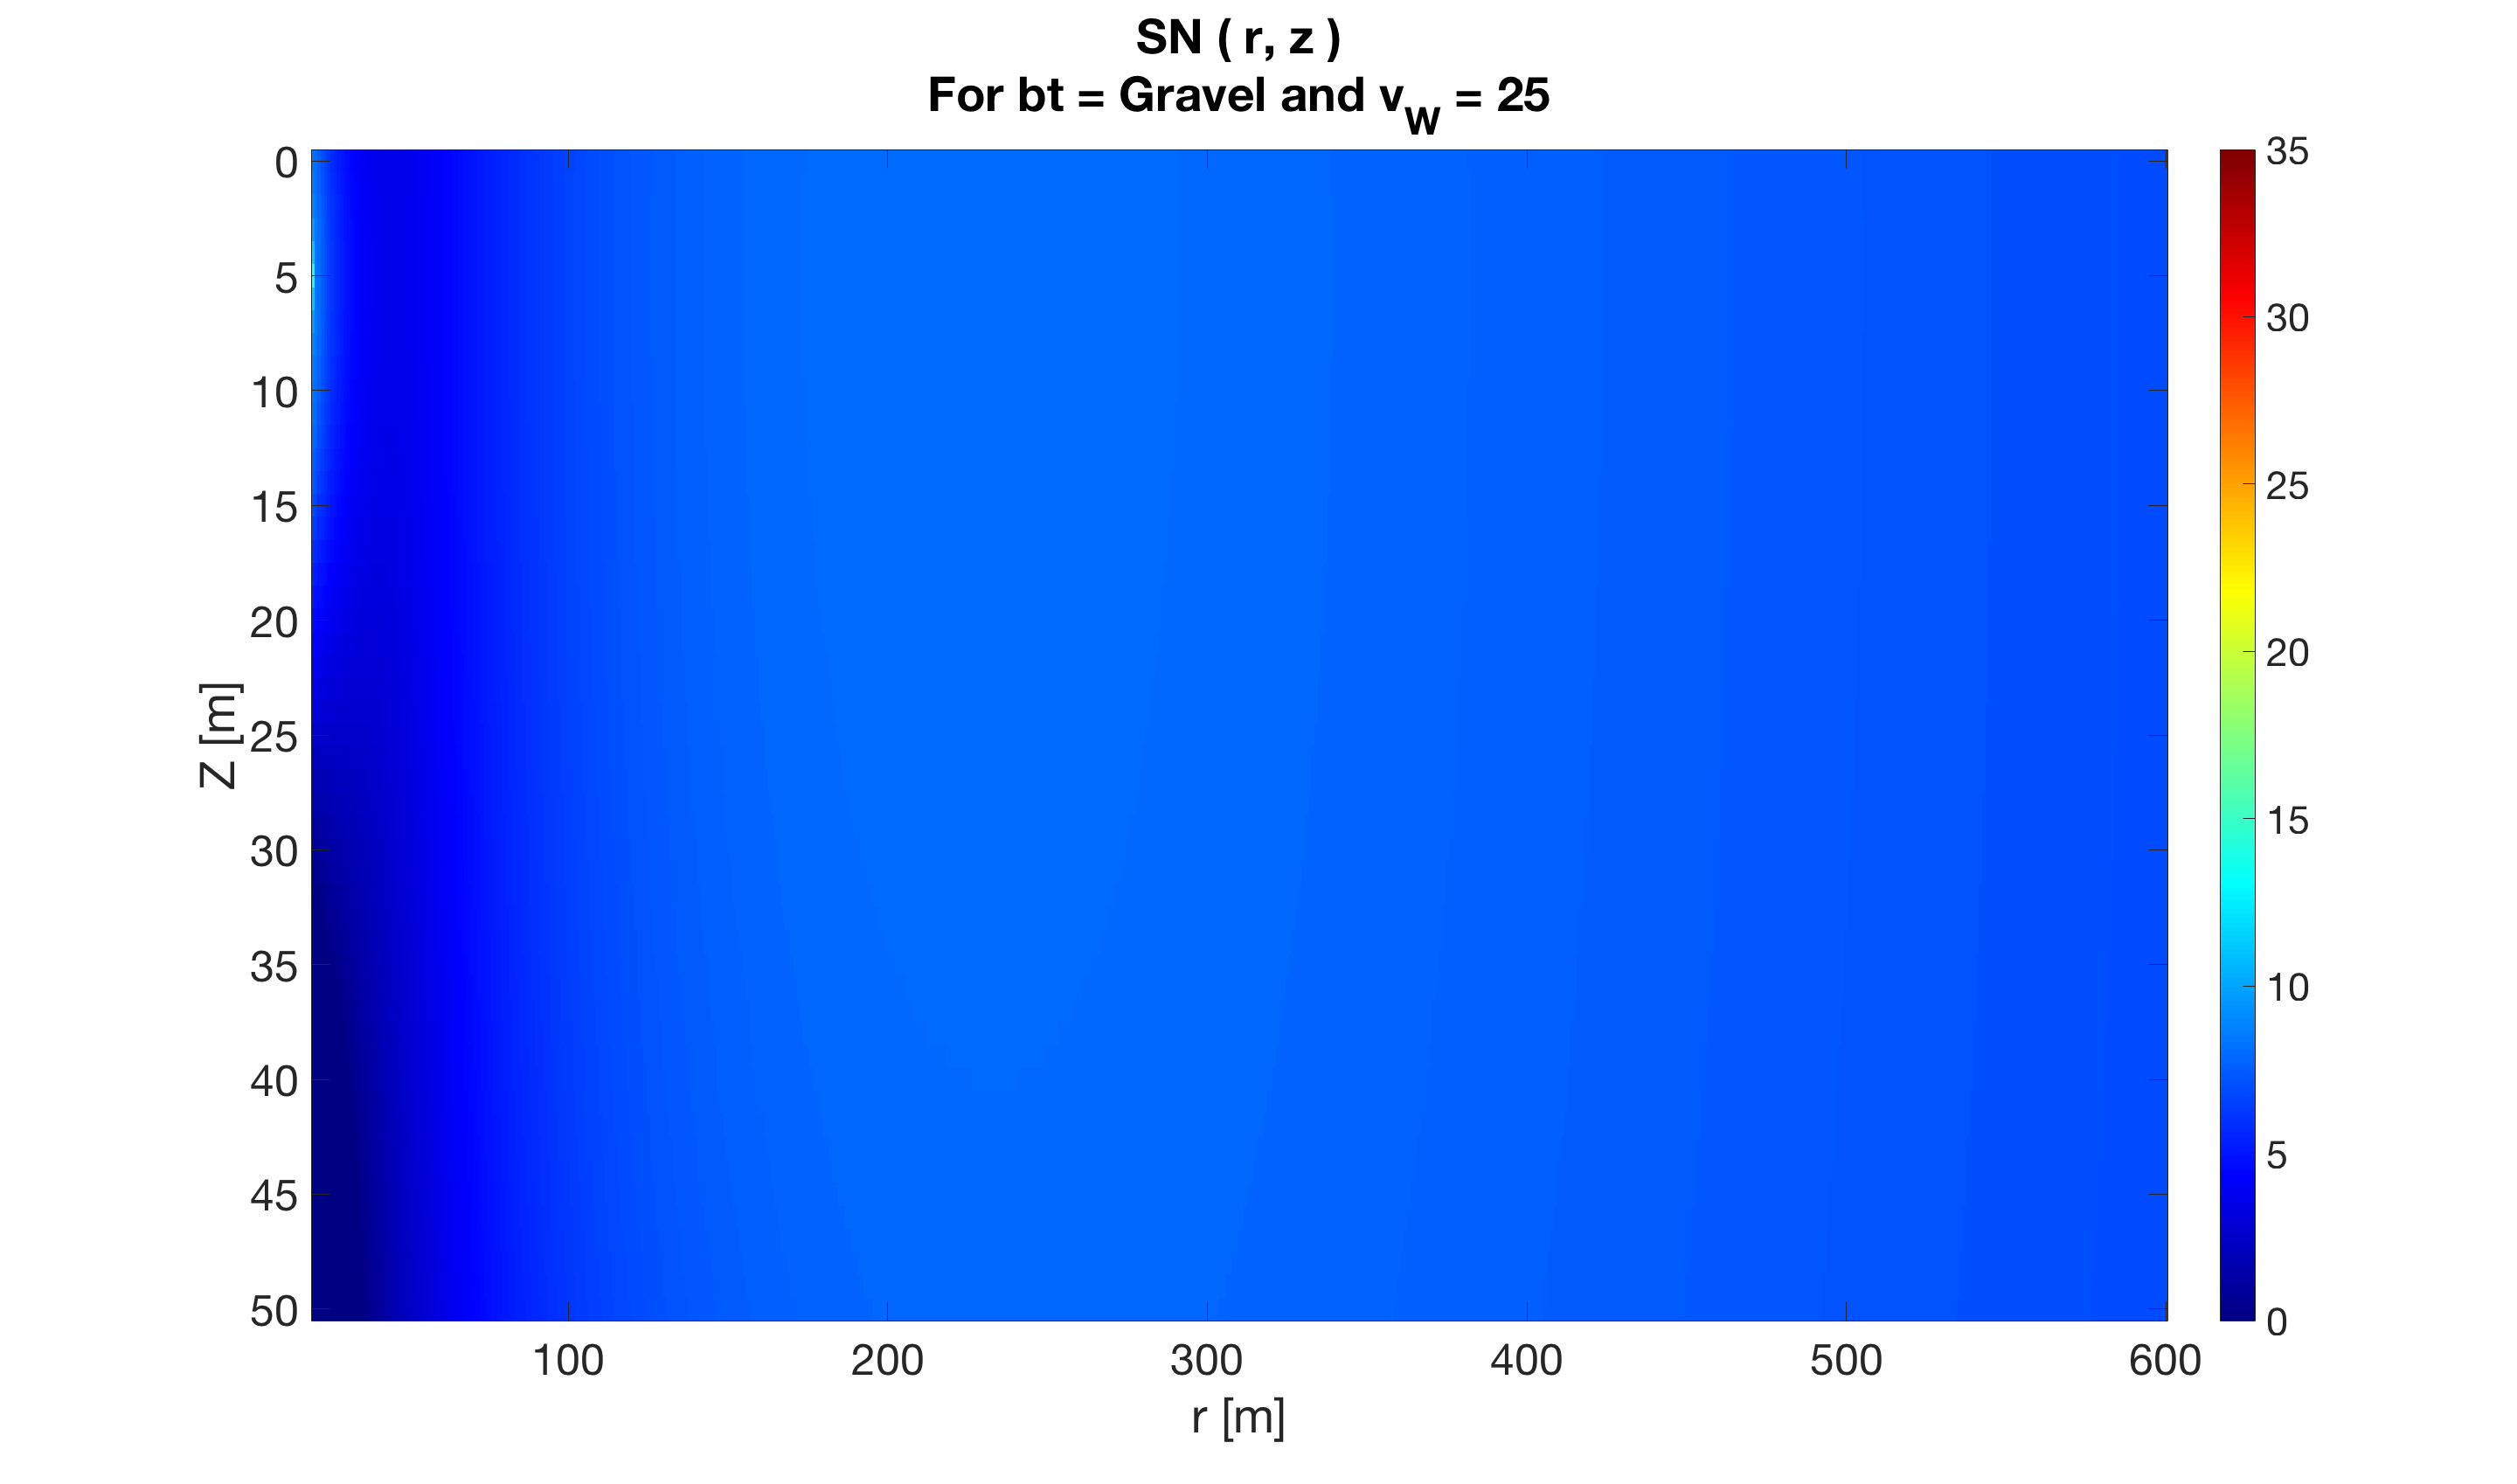
\includegraphics[width=90mm]{fig9.png}
}
\caption{Impact of gravel as the bottom type and wind speed of 5, 15 and 25 knots on the signal to noise ratio}
\end{figure}

\noindent As the bottom type changes from mud to gravel (soft to hard), signal to noise ratio is decreases gradually. At low wind speed values, the bottom type plays a vital role in determining SNR. For the bottom type of mud, SNR is decreasing with increasing wind speeds. For the hard bottom types with the high wind speeds, SNR will be worst. The SNR has medium values for the highest values of the bottom type mud and sand. For the bottom type gravel, the SNR has the smallest values i.e. SNR is getting worse and we can observe highest noise.


